

\begin{figure}[ht]
    \captionsetup[subfigure]{justification=centering}
    \centering
    \begin{subfigure}[b]{0.3\textwidth}
        \centering
        \includegraphics[width=0.475\textwidth]{figures/flatconnectordatasetimages/cut_corner_image.png}
        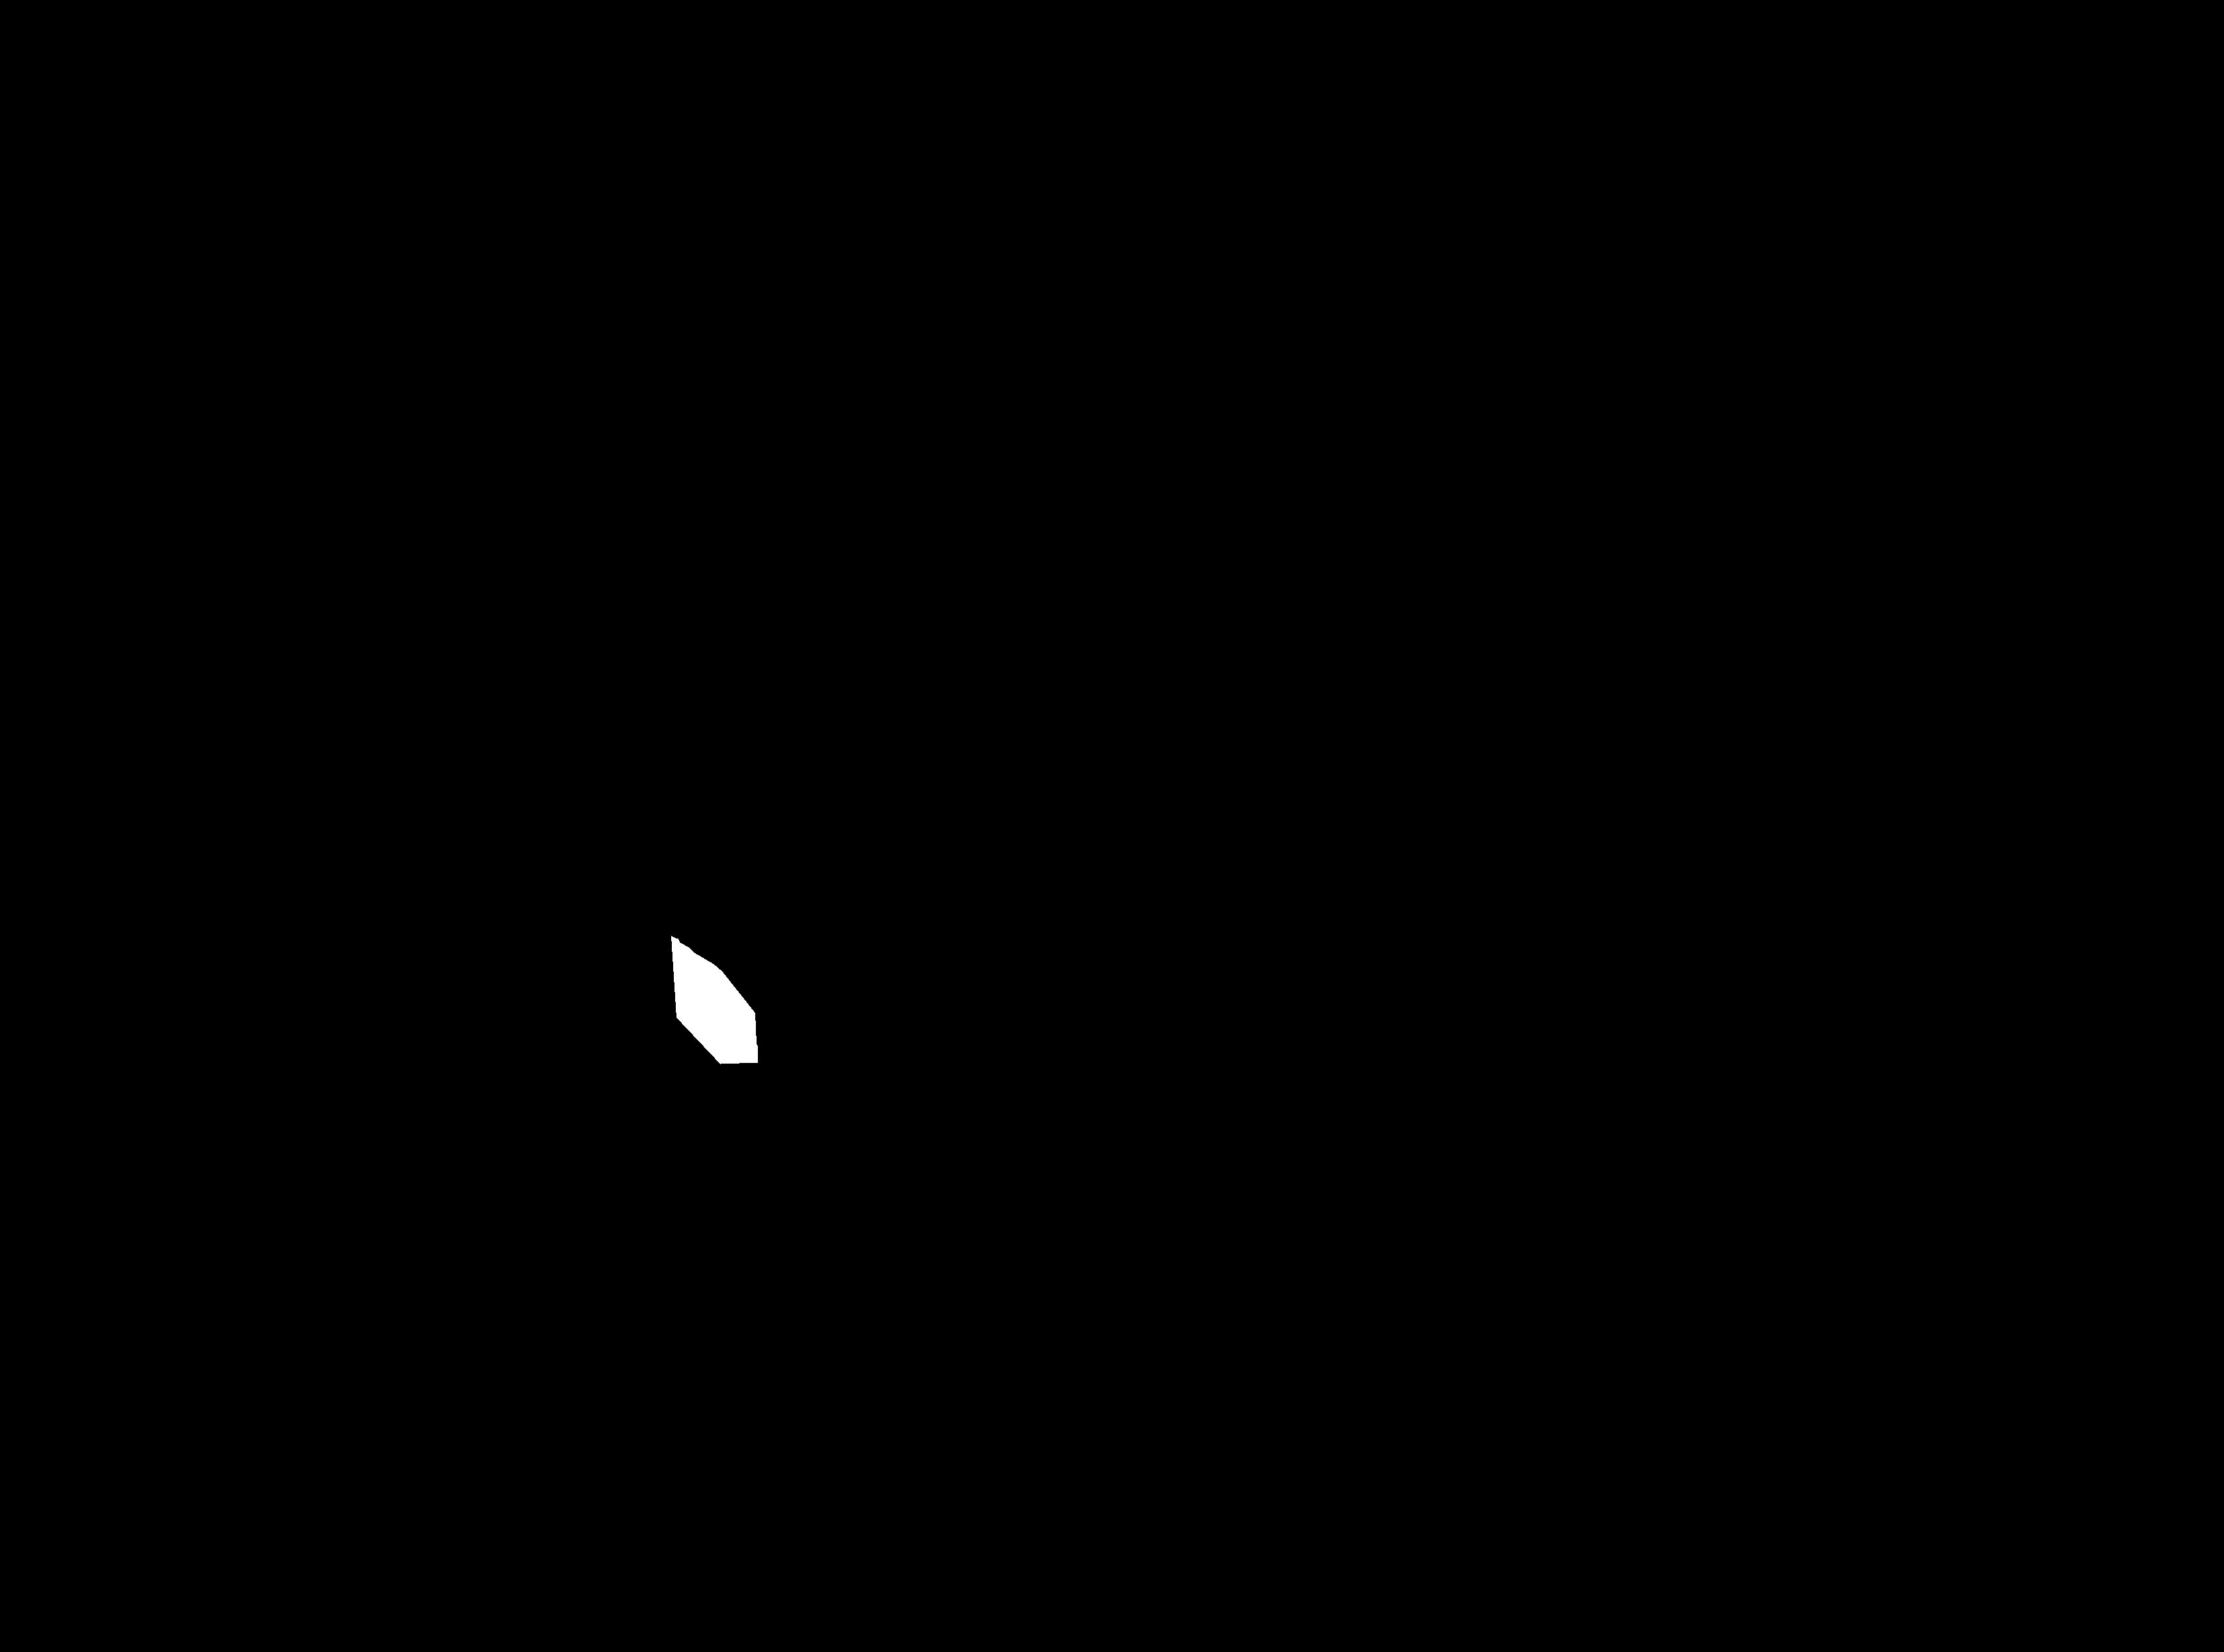
\includegraphics[width=0.475\textwidth]{figures/flatconnectordatasetimages/cut_corner_mask.png}
        \caption{Cut Corner}

    \end{subfigure}
    \hfill
    \begin{subfigure}[b]{0.3\textwidth}
        \centering
        \includegraphics[width=0.475\textwidth]{figures/flatconnectordatasetimages/damaged_edge.png}
        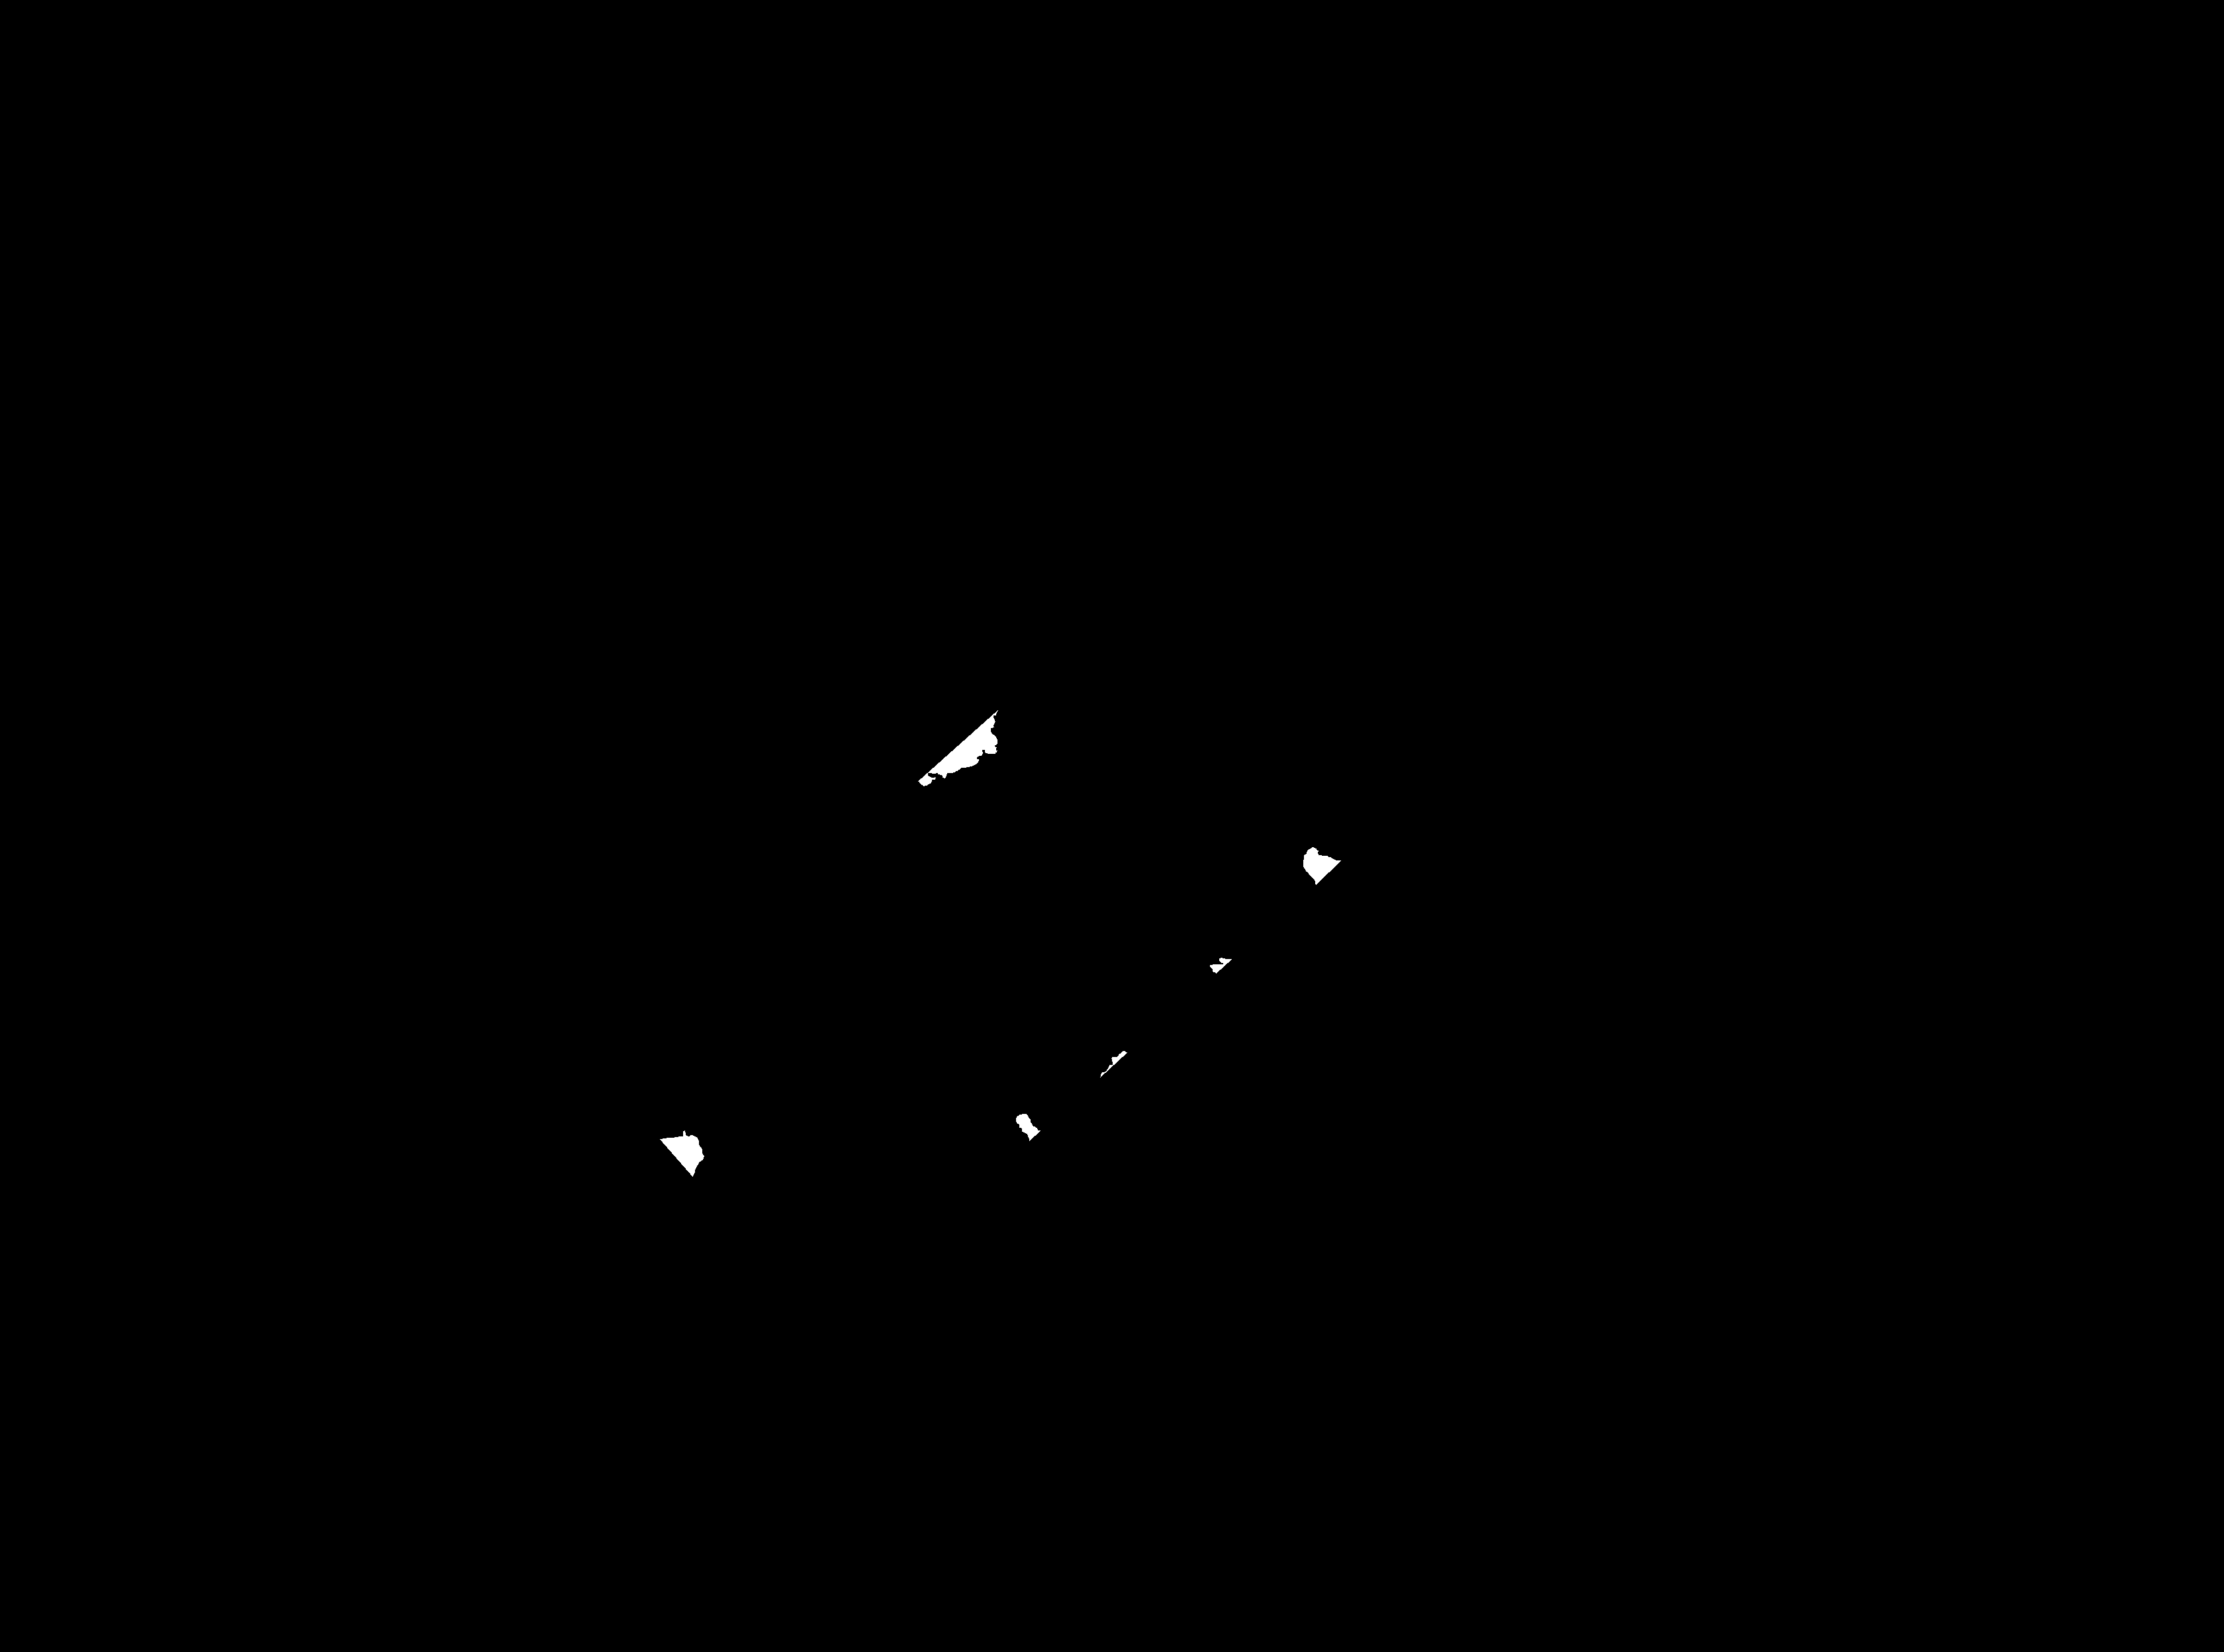
\includegraphics[width=0.475\textwidth]{figures/flatconnectordatasetimages/damaged_edge_mask.png}
        \caption{Damaged Edge}
        \label{fig:damagededgesubfig}
    \end{subfigure}
    \hfill
    \begin{subfigure}[b]{0.3\textwidth}
        \centering
        \includegraphics[width=0.475\textwidth]{figures/flatconnectordatasetimages/scratch.png}
        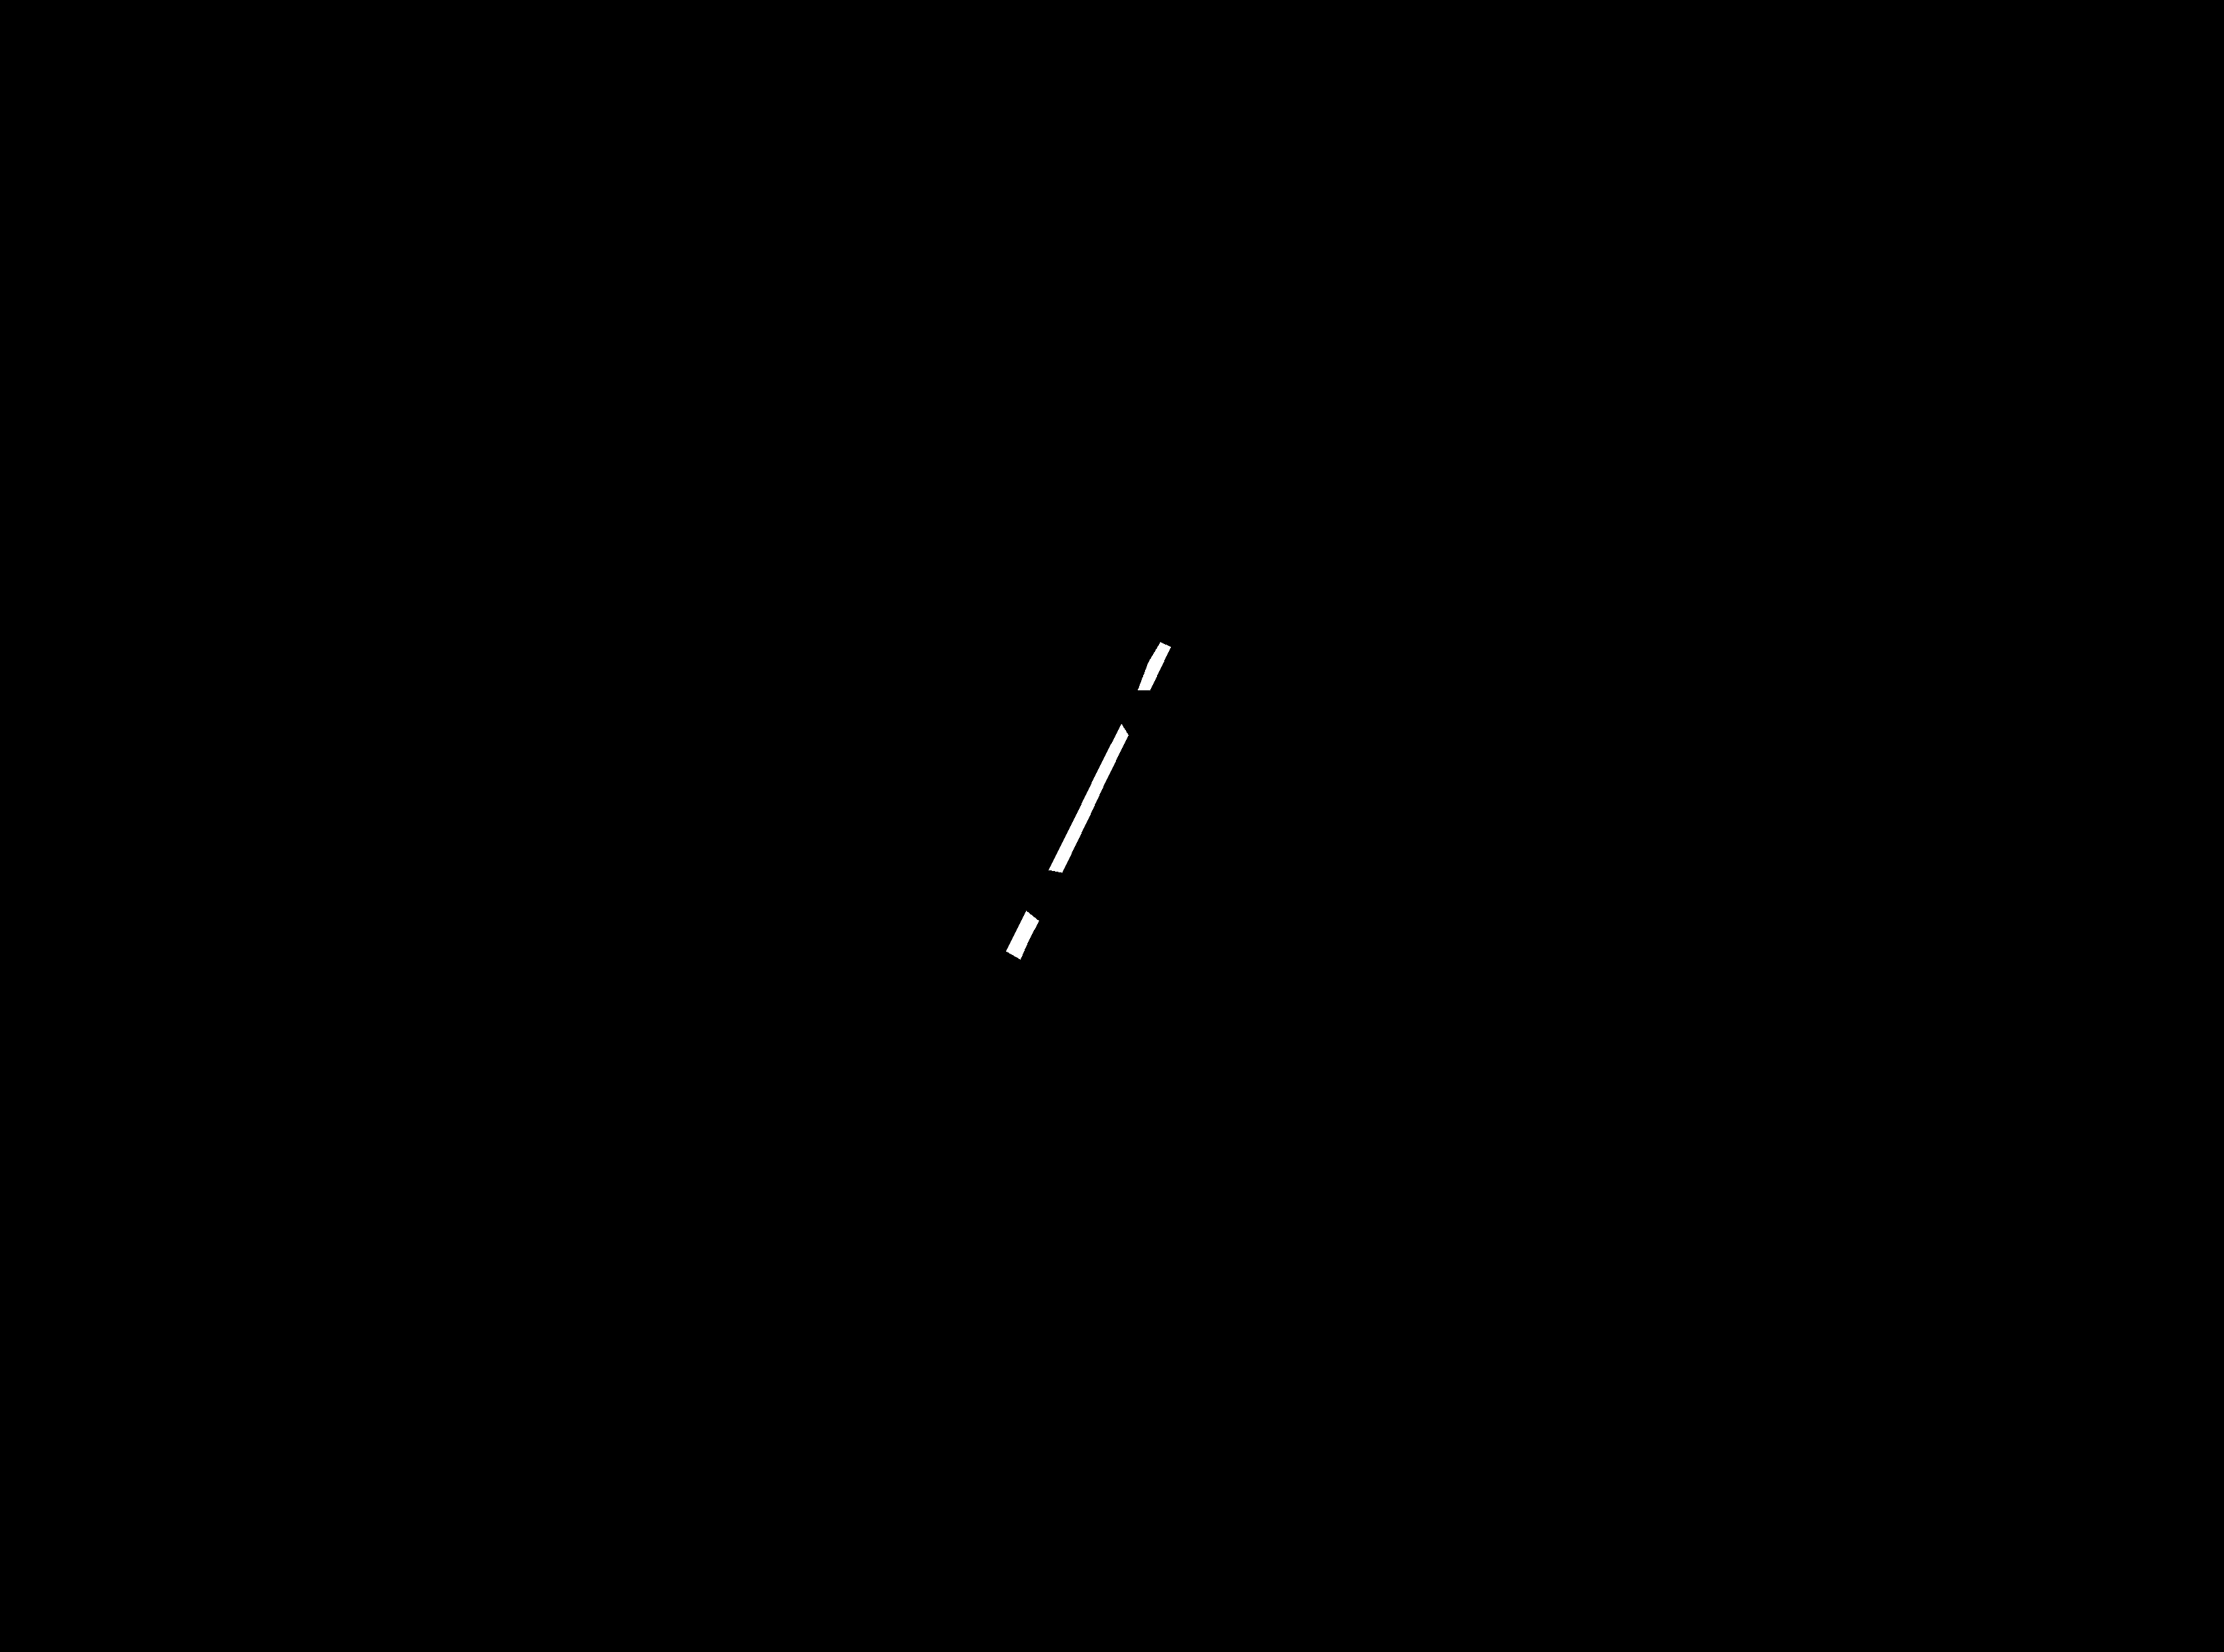
\includegraphics[width=0.475\textwidth]{figures/flatconnectordatasetimages/scratch_mask.png}
        \caption{Scratch}

    \end{subfigure}
    \\
    \begin{subfigure}[b]{0.3\textwidth}
        \centering
        \includegraphics[width=0.475\textwidth]{figures/flatconnectordatasetimages/missing_big_hole.png}
        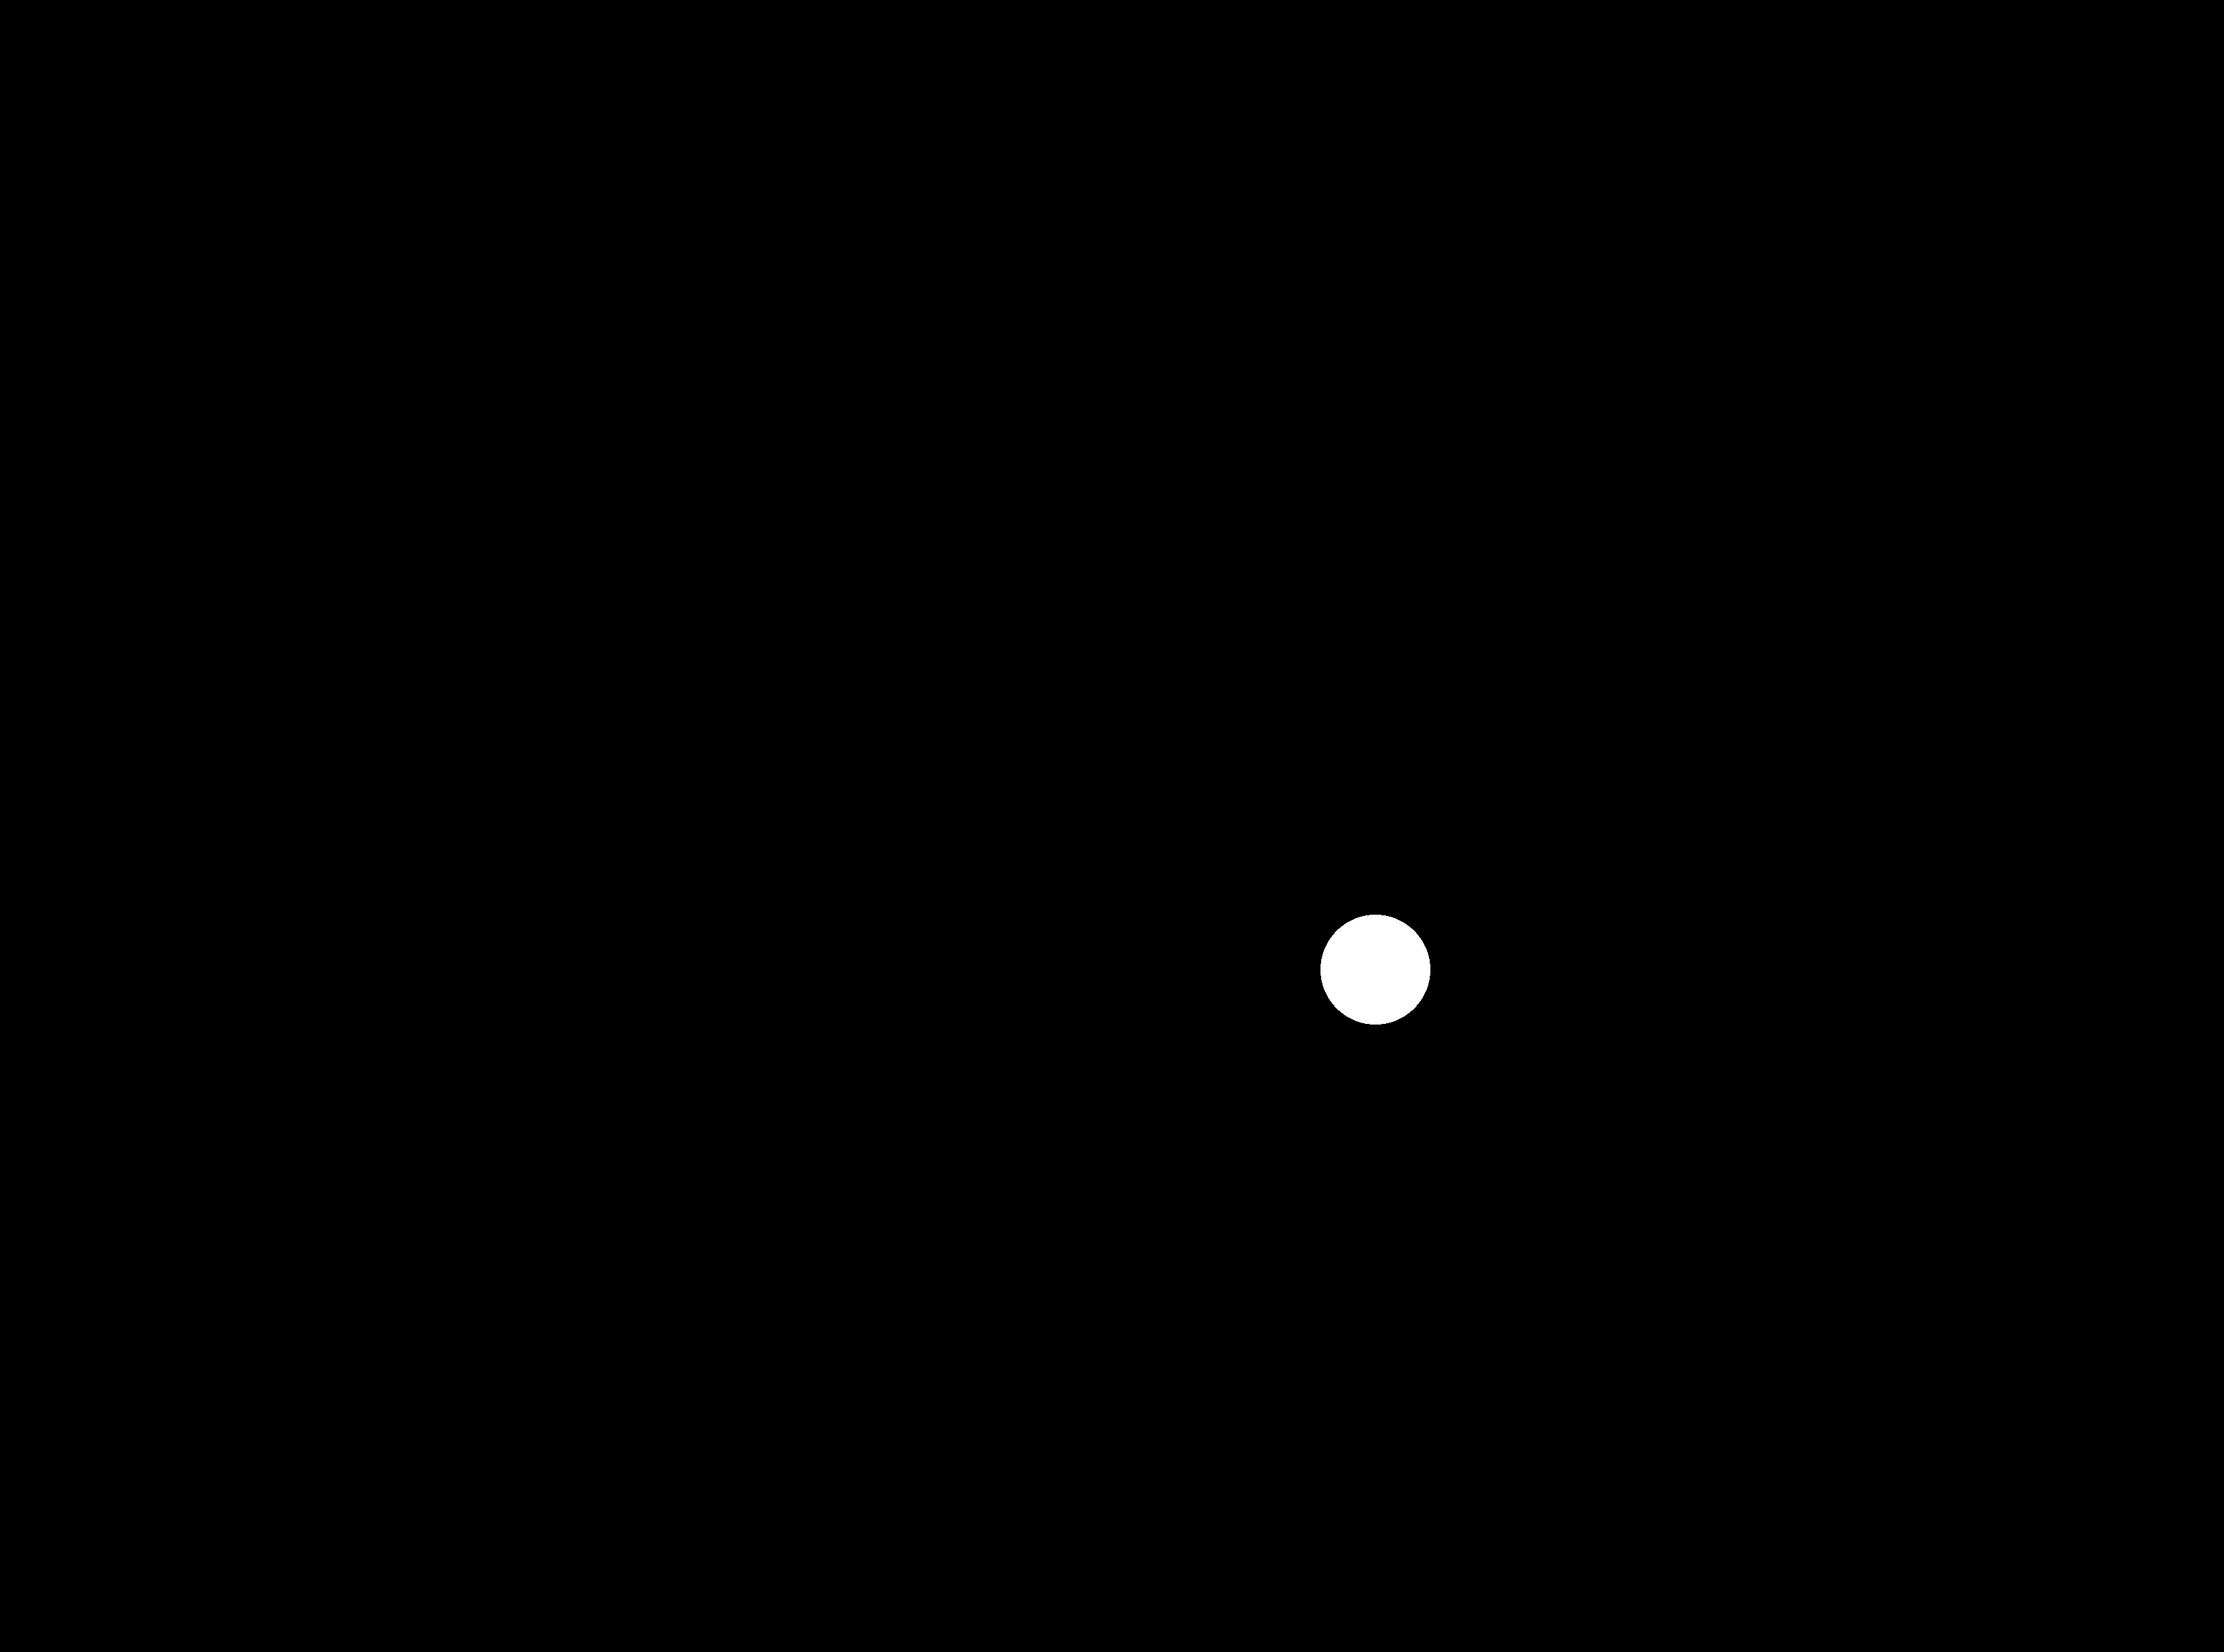
\includegraphics[width=0.475\textwidth]{figures/flatconnectordatasetimages/missing_big_hole_mask.png}
        \caption{Missing Big Hole}

    \end{subfigure}
    \hfill
    \begin{subfigure}[b]{0.3\textwidth}
        \centering
        \includegraphics[width=0.475\textwidth]{figures/flatconnectordatasetimages/extra_holes.png}
        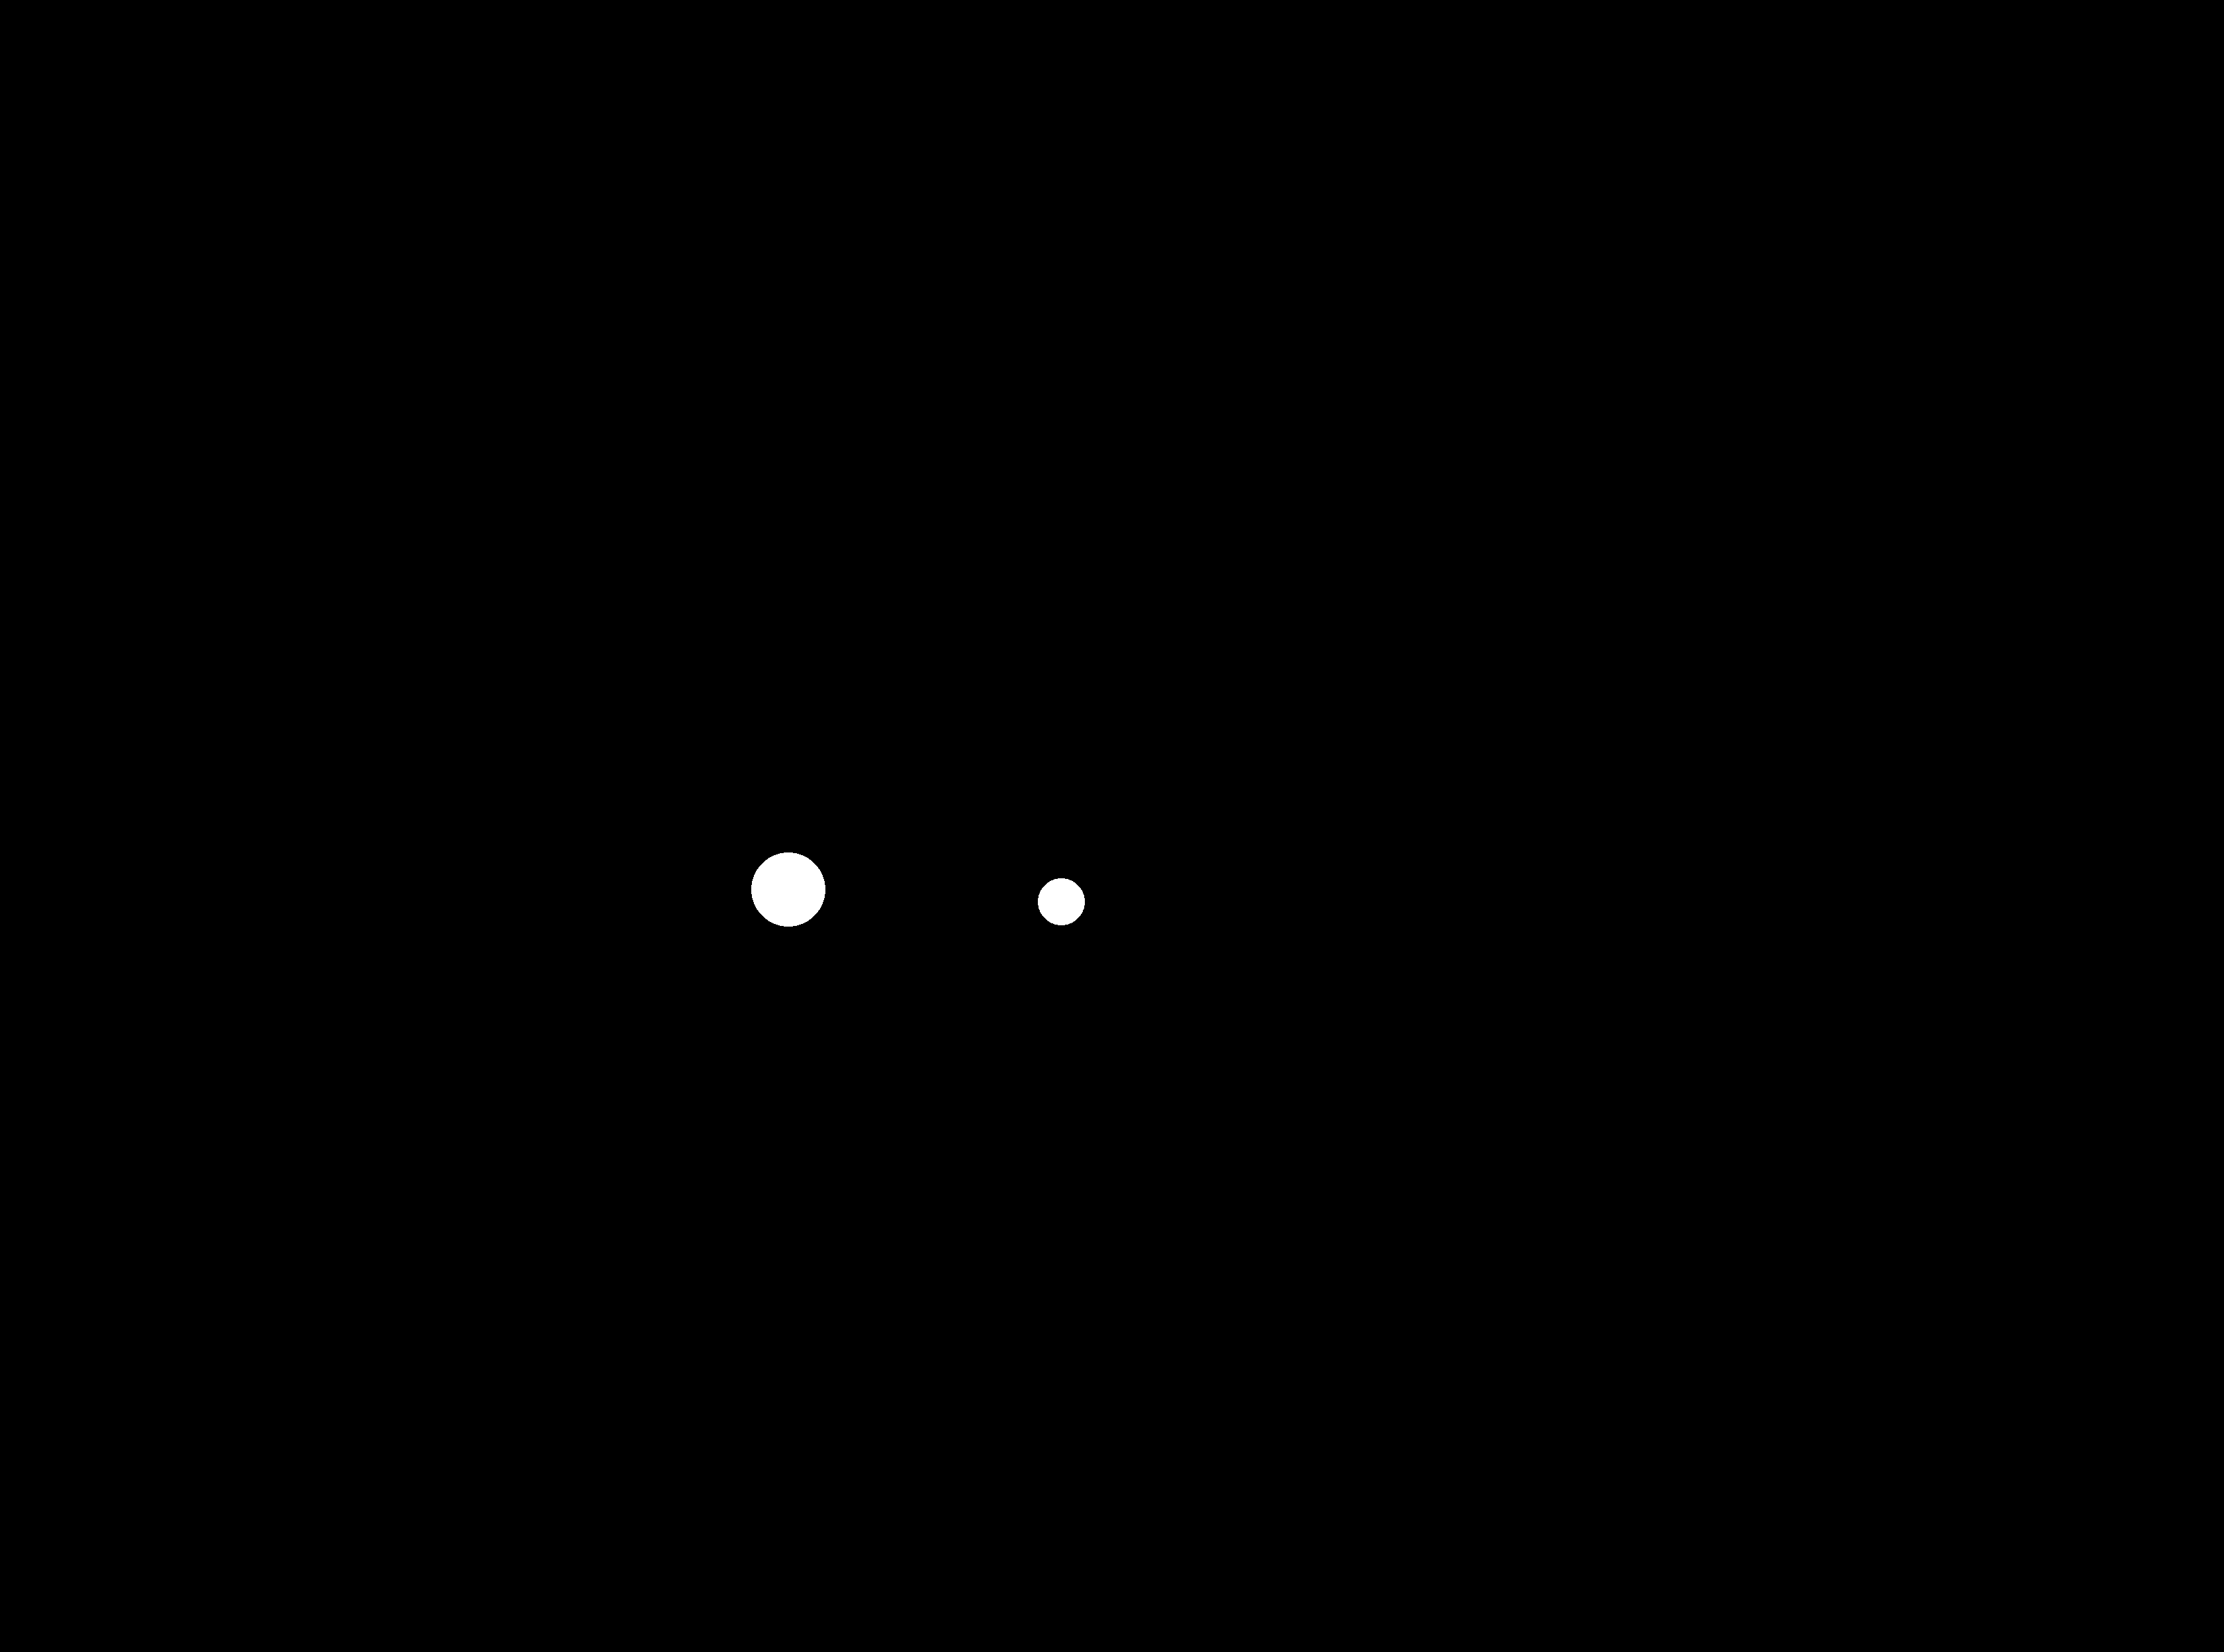
\includegraphics[width=0.475\textwidth]{figures/flatconnectordatasetimages/extra_holes_mask.png}
        \caption{Extra Holes}

    \end{subfigure}
    \hfill
    \begin{subfigure}[b]{0.3\textwidth}
        \centering
        \includegraphics[width=0.475\textwidth]{figures/flatconnectordatasetimages/diff_size_holes.png}
        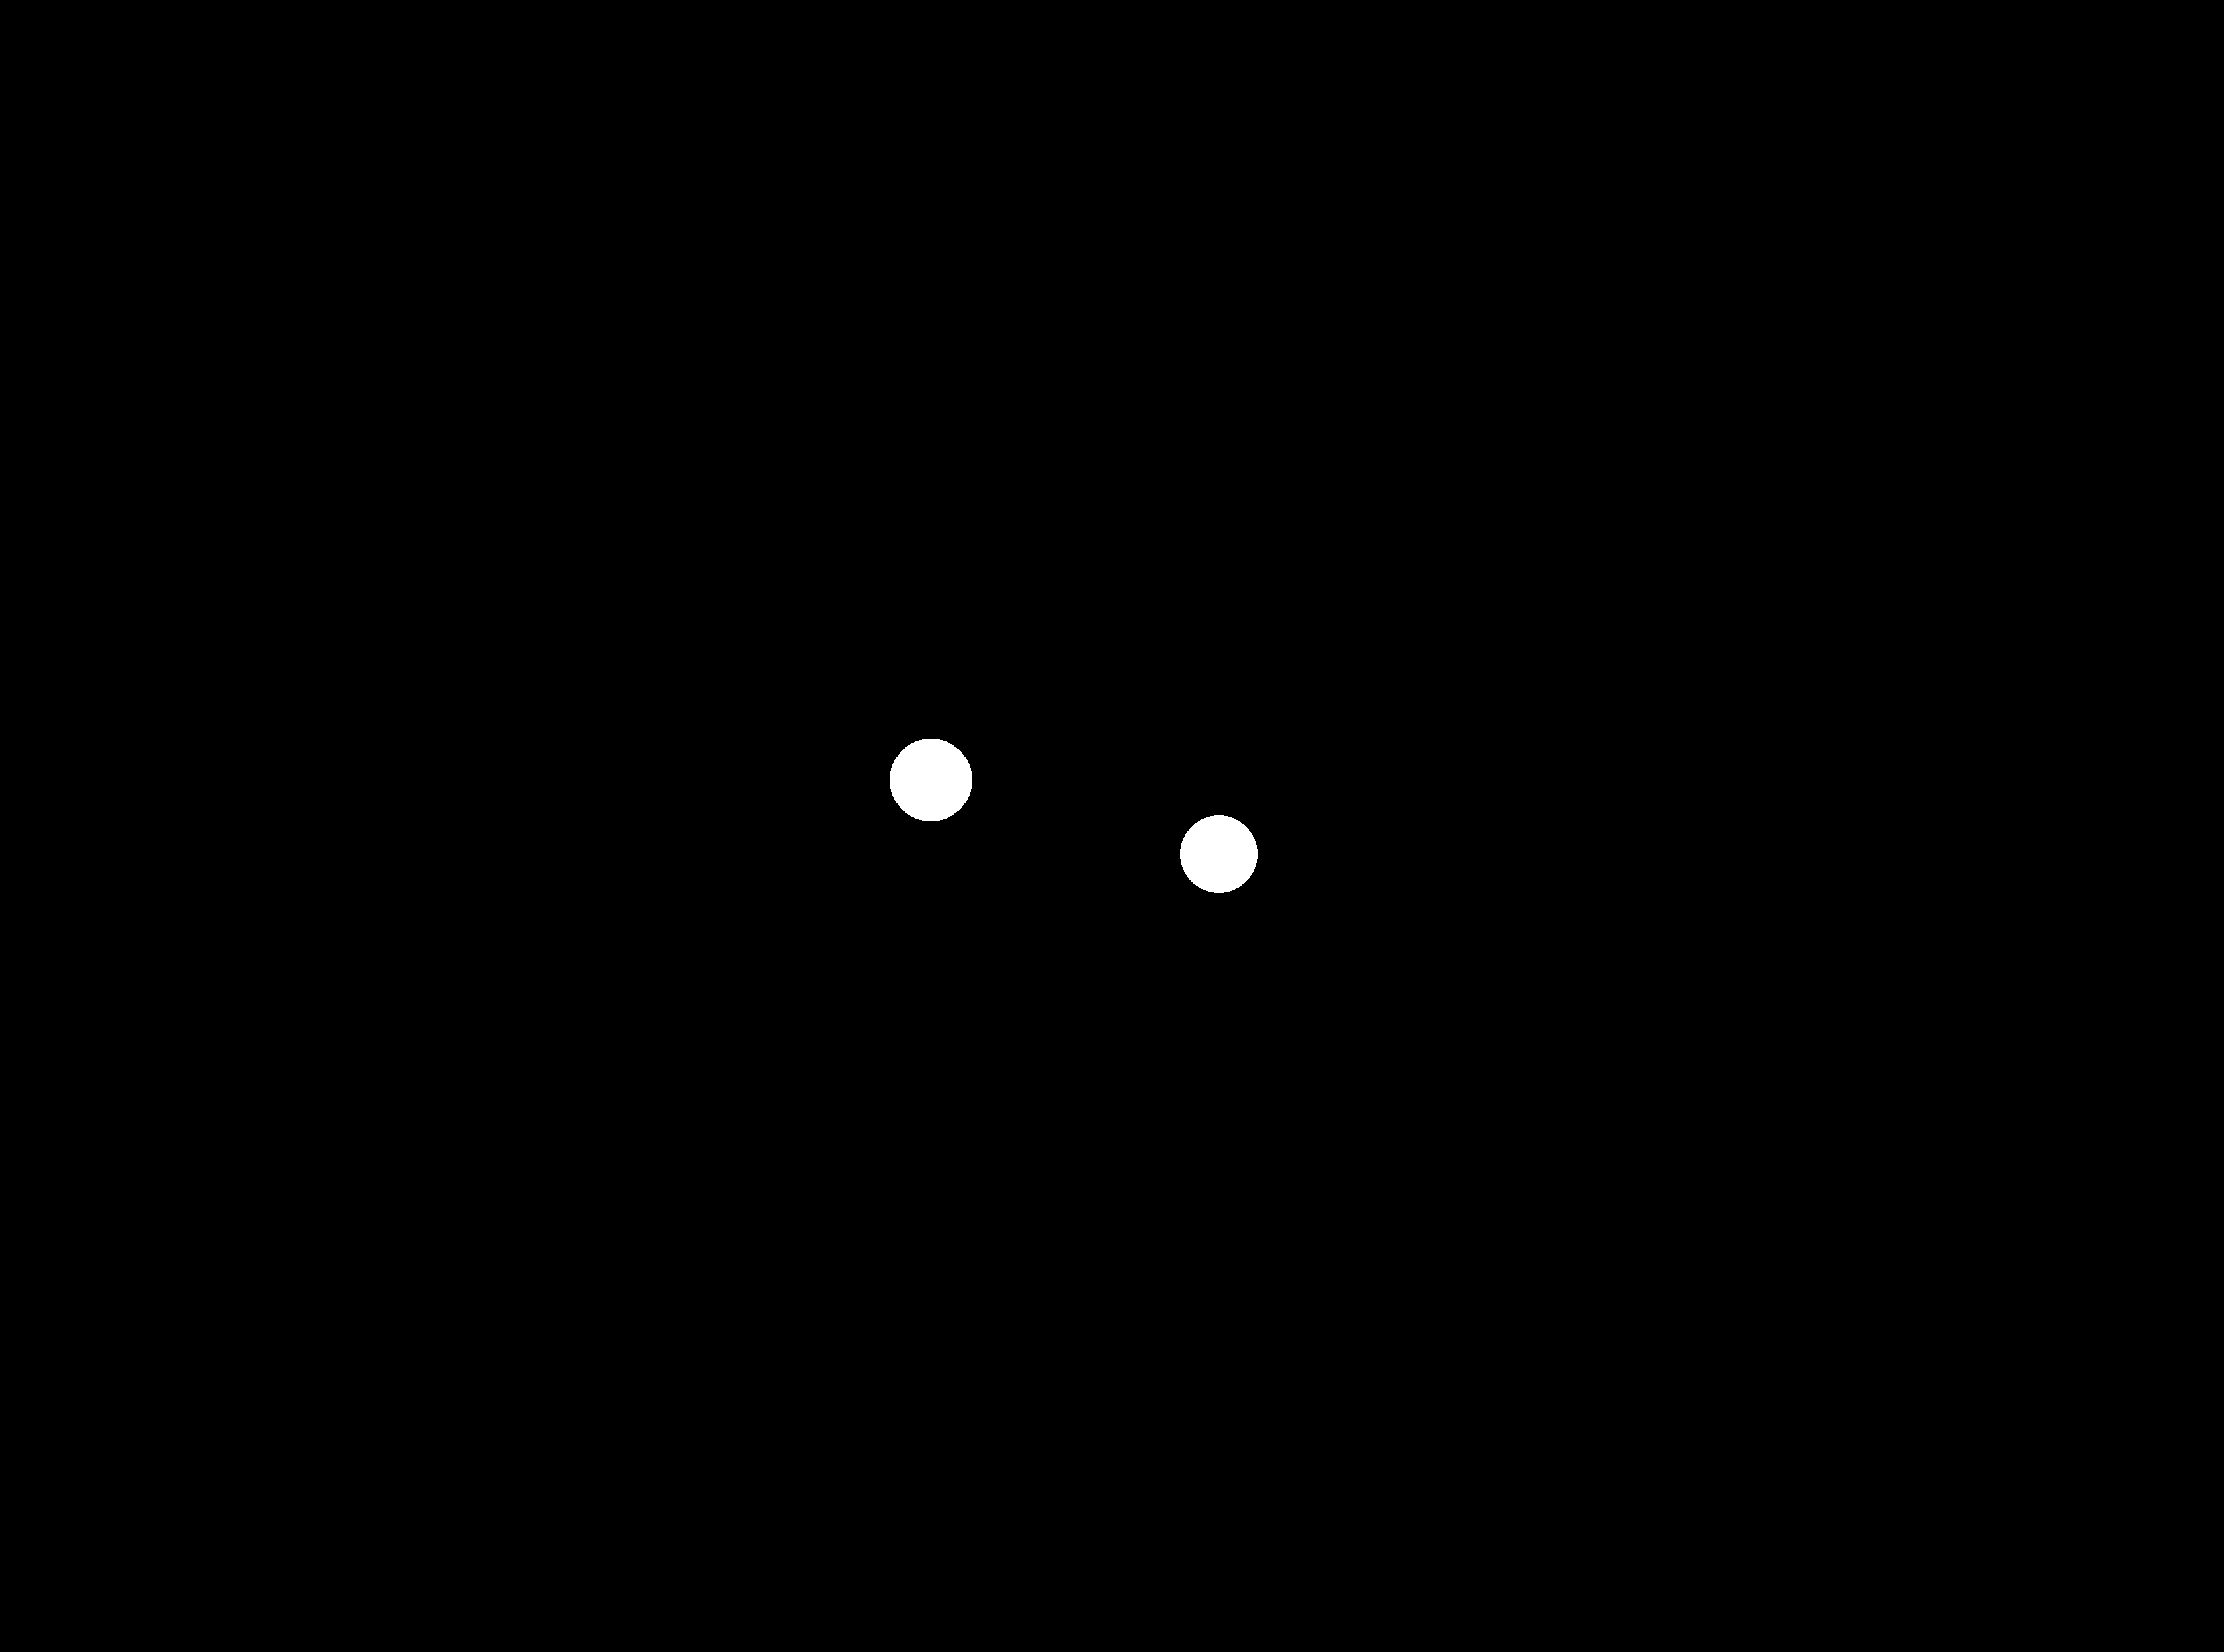
\includegraphics[width=0.475\textwidth]{figures/flatconnectordatasetimages/diff_size_holes_mask.png}
        \caption{Differently Sized Holes}

    \end{subfigure}
    %\captionsetup{justification=centering, skip=-10pt}
    \caption{Example images of anomalous samples from the novel flat connector class. The according class names are written below the subfigures.}
    \label{fig:flatconnectorexampleimages}
\end{figure}


